%%%%%%%%%%%%%%%%%%%%%%%%%%%%%%%%%%%%%%%%%
% Structured General Purpose Assignment
% LaTeX Template
%
% This template has been downloaded from:
% http://www.latextemplates.com
%
% Original author:
% Ted Pavlic (http://www.tedpavlic.com)
%
% Note:
% The \lipsum[#] commands throughout this template generate dummy text
% to fill the template out. These commands should all be removed when 
% writing assignment content.mus
%
%%%%%%%%%%%%%%%%%%%%%%%%%%%%%%%%%%%%%%%%%

%----------------------------------------------------------------------------------------
%	PACKAGES AND OTHER DOCUMENT CONFIGURATIONS
%----------------------------------------------------------------------------------------

\documentclass{article}

%\usepackage[brazilian]{babel}
\usepackage[utf8]{inputenc}
\usepackage{fancyhdr} % Required for custom headers
\usepackage{lastpage} % Required to determine the last page for the footer
\usepackage{extramarks} % Required for headers and footers
\usepackage{graphicx} % Required to insert images
\usepackage{float}
\usepackage{listings}
\usepackage{amsmath}
\usepackage[colorlinks=true, pdfborder={0 0 0}, urlcolor=blue, linkcolor=black]{hyperref}

\graphicspath{ {img/} }

% Margins
\topmargin=-0.45in
\evensidemargin=0in
\oddsidemargin=0in
\textwidth=6.5in
\textheight=9.0in
\headsep=0.25in 

\linespread{1.1} % Line spacing

% Set up the header and footer
\pagestyle{fancy}
\lhead{\hmwkAuthorName} % Top left header
%\chead{\hmwkClass\ (\hmwkClassInstructor\ \hmwkClassTime): \hmwkTitle} % Top center header
\rhead{\hmwkTitle} % Top center header
%\rhead{\firstxmark} % Top right header
\lfoot{\lastxmark} % Bottom left footer
\cfoot{} % Bottom center footer
\rfoot{Page\ \thepage\ of\ \pageref{LastPage}} % Bottom right footer
\renewcommand\headrulewidth{0.4pt} % Size of the header rule
\renewcommand\footrulewidth{0.4pt} % Size of the footer rule

\setlength\parindent{0pt} % Removes all indentation from paragraphs

%----------------------------------------------------------------------------------------
%	DOCUMENT STRUCTURE COMMANDS
%	Skip this unless you know what you're doing
%----------------------------------------------------------------------------------------

% Header and footer for when a page split occurs within a problem environment
\newcommand{\enterProblemHeader}[1]{
\nobreak\extramarks{#1}{#1\ldots}\nobreak
\nobreak\extramarks{#1 (continuation)}{#1}\nobreak
}

% Header and footer for when a page split occurs between problem environments
\newcommand{\exitProblemHeader}[1]{
\nobreak\extramarks{#1 (continuation)}{#1}\nobreak
\nobreak\extramarks{#1}{}\nobreak
}

\setcounter{secnumdepth}{0} % Removes default section numbers
\newcounter{homeworkProblemCounter} % Creates a counter to keep track of the number of problems

\newcommand{\homeworkProblemName}{}
\newenvironment{homeworkProblem}[1][\arabic{homeworkProblemCounter}]{ % Makes a new environment called homeworkProblem which takes 1 argument (custom name) but the default is "Problem #"
\stepcounter{homeworkProblemCounter} % Increase counter for number of problems
\renewcommand{\homeworkProblemName}{#1} % Assign \homeworkProblemName the name of the problem
\section{\homeworkProblemName} % Make a section in the document with the custom problem count
\enterProblemHeader{\homeworkProblemName} % Header and footer within the environment
}{
\exitProblemHeader{\homeworkProblemName} % Header and footer after the environment
}

\newcommand{\problemAnswer}[1]{ % Defines the problem answer command with the content as the only argument
\noindent\framebox[\columnwidth][c]{\begin{minipage}{0.98\columnwidth}#1\end{minipage}} % Makes the box around the problem answer and puts the content inside
}

\newcommand{\homeworkSectionName}{}
\newenvironment{homeworkSection}[1]{ % New environment for sections within homework problems, takes 1 argument - the name of the section
\renewcommand{\homeworkSectionName}{#1} % Assign \homeworkSectionName to the name of the section from the environment argumen
\subsection{\homeworkSectionName} % Make a subsection with the custom name of the subsection
\enterProblemHeader{\homeworkProblemName\ [\homeworkSectionName]} % Header and footer within the environment
}{
\enterProblemHeader{\homeworkProblemName} % Header and footer after the environment
}
   
%----------------------------------------------------------------------------------------
%	NAME AND CLASS SECTION
%----------------------------------------------------------------------------------------

\newcommand{\hmwkTitle}{Proposal for Bachelor Thesis} % Assignment title
\newcommand{\hmwkDueDate}{08 November 2014} % Due date
\newcommand{\hmwkClass}{} % Course/class
\newcommand{\hmwkClassFull}{} % Course/class
\newcommand{\hmwkClassTime}{} % Class/lecture time
\newcommand{\hmwkClassInstructor}{} % Teacher/lecturer
\newcommand{\hmwkAuthorName}{William Bombardelli da Silva} % Your name

%----------------------------------------------------------------------------------------
%	TITLE PAGE
%----------------------------------------------------------------------------------------

\title{
%\vspace{2in}
\Large\textmd{\textbf{\hmwkClassFull}}\\
\normalsize{\textbf{\hmwkTitle}}\\
\normalsize\vspace{0.1in}\small{\hmwkDueDate}\\
%\vspace{0.1in}
\large{\textit{\hmwkClassInstructor\ \hmwkClassTime}}
%\vspace{3in}
}

\author{\textbf{\hmwkAuthorName}}
\date{} % Insert date here if you want it to appear below your name

%----------------------------------------------------------------------------------------

\begin{document}

%\maketitle
{\centering
\Large\textmd{\textbf{\hmwkClassFull}}\\
\normalsize{\textbf{\hmwkTitle}}\\
\normalsize\vspace{0.1in}\small{\hmwkDueDate}\\
%\vspace{0.1in}
\large\textbf{\hmwkAuthorName}
%\large{\textit{\hmwkClassInstructor\ \hmwkClassTime}}\\

}
%----------------------------------------------------------------------------------------
%	TABLE OF CONTENTS
%----------------------------------------------------------------------------------------

%\setcounter{tocdepth}{1} % Uncomment this line if you don't want subsections listed in the ToC

%\newpage
%\tableofcontents
%\newpage

% To have just one problem per page, simply put a \clearpage after each problem

\begin{homeworkProblem}[Towards Synchronizing Relations Between Artifacts in the Java Technological Space]
	\begin{section}{Introduction}
	This document intents to describe the proposal for bachelor thesis by William Bombardelli da Silva, student of Informatik Bachelor in the Technische Universität Berlin, student number 364927.
	
	The goal of this bachelor thesis is to report the current state of research and to develop new contributions both theoretical and practical. By being so, the thesis aims to investigate a problem of software model synchronization in the context of Model-driven Engineering. More specifically the problem of defining relations between common software meta-models, in order to maintain their models synchronized is to be tackled.
	\end{section}
	
	\begin{section}{Key-words}
	Model Synchronization, Iterative Model Transformation, Model Transformation, Model Evolution, Model Co-evolution, Model-driven Engineering, Software Engineering.
	\end{section}	
	
	\begin{section}{Theme Description}
	Recent techniques of software engineering have been using the concept of software models in the construction of software systems. According to \cite{czarnecki2006feature} "\textit{Models are system abstractions that allow developers and other stakeholders to effectively address concerns, such as answering a question about the system or effecting a change}”. By defining a model as a system abstraction, it becomes clear, that a software system might have several models abstracted from it, each one representing certain aspects of the whole system. These models also have relations between them, in the sense that they all are supposed to describe the actual system consistently by not presenting logical contradictions. Here examples of models are \emph{UML class diagram}, \emph{Use Cases}, or even the source-code itself.
	
	The constant evolving nature of current large-scale software systems causes its models to be constantly changed. But in order to maintain this whole network of interconnected models consistent the changes have to be forwarded through the network, i.e. all models have to be synchronized. Suppose one have a \emph{UML Class Diagram}, a series of \emph{UML Sequence Diagrams} and the source-code. If a method has its name changed in the class diagram, all occurrences of this method has to have its name updated in the sequence diagrams and in the source-code. It turns out though, that neither a model synchronization tool comprising the most common meta-models used nowadays has been developed nor are clearly defined relation definitions between them available on literature. 
	
	The goal of this bachelor thesis is therefore first to choose software meta-models commonly used in current Java object oriented software systems, defining the meta-model definitions; second to define (or write) the relations between the chosen meta-models; and last, to showcase how these artifacts can be synchronized in some representative cases.
	
	In the end of this thesis development it is expected the creation of a report comprising the difficulties found and the next challenges for the problem. The meta-models used might be narrowed to \emph{MOF} compliant (see \cite{omg2015meta}) meta-models.
	\end{section}
	
	\begin{section}{Motivation}
	The lack of a functional model synchronization tool integrating a broad range of meta-models used currently in software engineering is the main motivation for this thesis. Although an expressive effort has been made by the academic community to create solutions for the problem of model synchronization, no study known by us presents an effective tool, that could be used extensively in practice. We believe though, that the contribution of this thesis can be useful for the creation of such a tool.
	
	Another motivation for this thesis is the lack of relation definitions in current literature for extensively used meta-models in industry. Examples of these relations include relations between \emph{UML Class and Sequence Diagrams} and \emph{Java Code}, between \emph{Use Cases} and \emph{Requirements Diagrams}, between \emph{OCL contracts (used in design by contract methods)} and \emph{Unit Tests}, among others. It means, that the success of this thesis might bring the contribution towards the definition of a network of interconnected meta-models useful to both research and industry community. Therefore the availability of such a network might finally allow the extensive use of Model-driven Engineering in practice $-$ helping bridging the gap between system abstractions and their concrete form $-$ and the further development of more sophisticated model synchronization methods.
	
	It is worth to note also, that the contribution of this thesis might help enhancing the quality of current software construction and therefore lessening the number of software problems and errors, what is an endemic problem nowadays, by fomenting the wide application of Model-Driven Software Development.
	\end{section}
	
	\begin{section}{State of Current Research}
	A research road-map for model synchronization found in France and Rumpe \cite{france2007model} gives an overview on the realm, and an interesting point of view about the challenges. In Mens and Van Gorp \cite{mens2006taxonomy} a taxonomy for model transformation is proposed, what helps to carry more precise analysis. In Czarnecki and Helsen \cite{czarnecki2006feature} a survey was driven and a framework for classification of model transformation approaches was presented.
	In Diskin et al \cite{diskin2014towards} a taxonomy for a network of models is presented and in Diskin \cite{diskin2011model} a theoretical algebraic basis is proposed.
	
	Between the attempts to build a model synchronization tool are the \emph{ATL Eclipse Plug-in} \cite{jouault2008atl}, which uses the \emph{Atlas Transformation Language to code the relations between models; the Medini QVT \footnote{http://projects.ikv.de/qvt}, which claims to implement the \emph{Query/View/Transformation Language} to code the relations; and the FUJABA \cite{nickel2000fujaba}, in which relations are coded using \emph{Triple Graph Grammars}.} Other publications aim to solve specific problems, like the ones in Hermann et al \cite{hermann2011correctness}, Xiong et al \cite{xiong2007towards}, Giese and Wagner \cite{giese2006incremental}, Ivkovic and Kontogiannis \cite{ivkovic2004tracing}, or Song et al \cite{song2011instant}, where advanced algorithms for bidirectional synchronization have been proposed. But none of the above have accomplished to develop an extensible and efficient tool capable of integrating the most used types of meta-models.
	
	Nevertheless, recently Käfer et al have published their work on the \emph{CoWolf Framework}, which is "\textit{an extensible framework for model evolution and co-evolution management}" \cite{getir2015cowolf}. Although the number of supported meta-models is rather small, the extensibility claimed by them and the brief analysis we have made indicate us, that it is a promising option. The \emph{CoWolf} is built as a Eclipse plug-in, that employs other Eclipse plug-ins, all of them supported by the community; uses \emph{EMF} \cite{steinberg2008emf} to code the meta-models; and uses \emph{Henshin} \cite{arendt2010henshin} to code their relations.
	
	Additionally, one can judge by the date of publication of these works, that the topic of model synchronization is extremely active and is actually the edge of current academic research, what motivates even more the development of this thesis.
	\end{section}
	
	\begin{section}{Concepts Definition}
	Below is a list of necessary basic concepts, that will be used throughout this document.
	
	\textbf{Model:} The definition for software model used is: “Models are system abstractions that allow developers and other stakeholders to effectively address concerns, such as answering a question about the system or effecting a change” \cite{czarnecki2006feature} Examples of models, according to this definition, are \emph{UML diagrams}, \emph{OCL expressions}, \emph{relational database diagrams}, or even source-code.
	
	\textbf{Modeling Language:} For the scope considered here, modeling language is broadly defined as a language used to create models, that can be textual or graphical and may occur in several paradigms. Among them, functional, declarative or operational paradigms.
	
	\textbf{Model Relation:} Model relation here is defined abstractly as every relationship or constraint possible to happen between one source model and one target model.
	
	\textbf{Model Transformation:} Model transformation can be viewed as common data transformation – very common in computer science – with the specificity of dealing with models \cite{czarnecki2006feature}. In these terms, one can see model transformation from several points of view, for example as a sequence of operations/modifications over one model; or as a function, whose inputs relate to initial models and the output reflect the updated models.
	
	\textbf{Model Synchronization:} The goal of model synchronization is to maintain all relations between the models of a system consistent/correct as updates are performed over them \cite{diskin2011model}. Model synchronization may be seen as a procedure, a series of model transformations; as a function, which output – e.g. consistent updated set of models – is determined by the inputs – e.g. consistent set of models plus transformations to be executed; or even as a relation between set of models.
	As model synchronization is a relative new field of study, no fixed definition or approach is consensus between researchers, what brings up a variety of possible strategies and conjectures to solve the problem.
	
	\textbf{Network of Models:} A network of models of a system $S$ is an undirected graph $G = (V,E)$, whereas each vertex $v_i \in V$ represents a unique model $i$ of $S$, and an edge $(v_i, v_j)$ exists if, and only if there is a relation defined between both models $i, j \in S$.
	
	%FIXME: Define Technological space 
	\end{section}
	
	\begin{section}{Problem Definition}
	The problem tackled in this thesis is first to identify currently commonly used meta-models in the Java technological space. Second to capture common relations between these meta-models. And third to showcase the synchronization of such relations in a tool.
	
	An example of a possible network of meta-models created by the end of this work is supposed to look basically like the figure \ref{fig:NetExample01}:
	\begin{figure}[H]
	\centering
	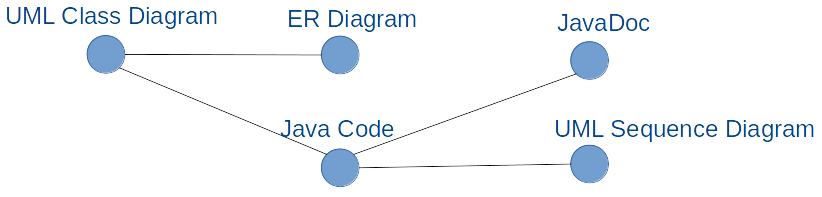
\includegraphics[scale=0.5]{NetworkExample_01}
	\caption{Example of a possible network of meta-models to be constructed. Like stated in the text, the meta-models are chosen accordingly basically to the frequency they are used currently in the Java technological space.}
	\label{fig:NetExample01}
	\end{figure}
	
	In the first moment the meta-models comprised in the network are to be defined, this is done through an extensive state-of-art research. So for example, in this phase the choice of applied meta-models (i.e. \emph{UML Class Diagram} and \emph{Java Code}) will be done and their definitions will be written. Possibly, simplifications on the meta-models shall be done, so that they fit the necessities of our scope, and can be made using the \emph{EMF} standard \cite{steinberg2008emf}.
	
	Later on, given the defined meta-models (this is the vertices of the network), their relations (this is the edges of the network) can be written, what can be made with Triple Graph Grammars. So for example, in this phase the inherent relation between the \emph{UML Class Diagram} meta-model and the \emph{Java Code} meta-model will be written. Analogously, the relations between \emph{Java Code}, \emph{JavaDoc}, \emph{UML Sequence Diagram} and other meta-models of the Java technological space can be also defined. Some of these relations might be found in current research literature, others might have to be invented during the development of this thesis.
	
	After having this network of meta-models ready, creating an actual network of more concrete models of any software system is trivial, thus study cases and example networks can be developed.
	
	The next step is then taken, and the synchronization of the created network of models is showed using a specific tool or method, which are to be chosen during the development of the thesis, so that the necessities can be accordingly fulfilled.
	
	In the end the result might be a network of meta-models useful in practice, in benchmarks and further researches as well. The showcase created will also be available as a possibly very useful tool. Furthermore, the report of this thesis recording the difficulties and experiences found during the work process and a possible analysis and discussion of future development is also supposed to be a legacy.
	\end{section}
	
	\begin{section}{Possible Difficulties}
	Possible difficulties that can be found throughout the development of this thesis include:
	\begin{itemize}
		\item The definition of the meta-models in the network of meta-models might be complicated and require relatively extensive work. For example, the definition of the \emph{Java Code} meta-model can be very broad and thus a narrowing of it is likely to be necessary.
		\item Some relations of the network might be difficult or complicated to build, requiring much time, so that it is not possible to include it in the scope of this thesis.
		\item Learning the Eclipse plug-ins like \emph{EMF} might represent some effort.
		\item Finding the best way to showcase the synchronization of the model network built might be the greatest challenge of this research and surely represents a danger.
	\end{itemize}
	\end{section}
	
	\begin{section}{Time Schedule}
	\begin{table}[H]
	\centering
	\begin{tabular}{l | l | l }
		\textbf{Duration} & \textbf{Start and End Dates} & \textbf{Activities} \\ \hline
			2 Weeks &	13/10/2015 to 26/10/2015 &	Initial research; definition of theme; finding of literature\\ \hline
			1 Weeks &	27/10/2015 to 02/11/2015 &	Detailed research; write of proposal; definition of scope\\ \hline
			2 Weeks &	03/11/2015 to 16/11/2015 &	Deepening in the theme; sketch of the development\\ \hline
			3 Weeks &	17/11/2015 to 07/12/2015 &	Analysis; design; pre-development phase; review; start of the writing\\ \hline
			5 Weeks &	08/12/2015 to 11/01/2016 &	Development; testing, validation and verification; review; writing\\ \hline
			2 Weeks &	12/01/2016 to 25/01/2016 &	Validation and verification; review; writing\\ \hline
			3 Weeks &	26/01/2016 to 15/02/2016 &	Finalization of writing; review\\ \hline
			1 Weeks &	16/02/2016 to 22/02/2016 &	Preparation of presentation\\ \hline
			1 Weeks &	23/02/2016 to 29/02/2016 &  Final review\\ \hline
	\end{tabular}
	\caption{Plan for the researching, developing and writing of the bachelor thesis. This schedule is organized in weeks, whereas each week has its respective activities planed.}
	\end{table}
	\end{section}
	
	\bibliographystyle{plain}
	\bibliography{bibliography}
	
\end{homeworkProblem}

\end{document}

